\documentclass[11pt, a4paper]{article}
\usepackage{graphicx} % Required for inserting images
\usepackage[colorlinks=true, allcolors=blue]{hyperref} %para linkear diferentes sitios
\graphicspath{{images/}} %comando para traer las imagenes
\usepackage{titlesec} %cambia el tamanio de fuente
\usepackage{fontspec} %Permite usar el mainfont
\usepackage{fancyhdr}
\pagestyle{fancy}

%tipo de fuente
\setmainfont{Times New Roman}

%tamanio de letras

\newcommand{\secfnt}{\fontsize{16}{19}} 
\newcommand{\ssecfnt}{\fontsize{14}{17}}

\renewcommand{\baselinestretch}{1,5} %interlineado

\renewcommand{\footrulewidth}{0pt}
\renewcommand{\headrulewidth}{0pt}

%pie de pagina
\lfoot{Basile , Colombo, 

de la Peña , Fittipaldi,

Garcia , Mancini,

Ordorica , Parrado,

Piñeiro , Saenz
}

\rfoot{\thepage}
\cfoot{}

%encabezado de la pagina
\fancyhead[C]{Byteados}
\fancyhead[R]{}

\titleformat{\section}
{\normalfont\secfnt\bfseries}{\thesection}{1em}{}

\titleformat{\subsection}
{\normalfont\ssecfnt\bfseries}{\thesubsection}{1em}{}


\title{Documentacion}
\author{Byteados}
\date{1er cuatrimetre 2024}

\begin{document}
\maketitle
\tableofcontents

\subsection{Enlaces externos:}

\begin{itemize}
    
\item \href{https://leafletjs.com/examples.html}{Leaflet}
\item \href{https://education.github.com/git-cheat-sheet-education.pdf}{GIT cheatsheet}
\item \href{https://docs.github.com/en/authentication/connecting-to-github-with-ssh}{GitHub SSH setup}
\item \href{https://flask.palletsprojects.com/en/3.0.x/}{Flask doc}
\end{itemize}

\section{Integrantes}

Listado de integrantes, padrón y su mail de contacto.
\begin{center}
\begin{tabular}{|c|c|c|}

   \hline\hline
   Jose Piñeiro Sanchez  & 106382 & @fi.uba.ar\\
   \hline
   Tomas Ordorica  & 111636 & @fi.uba.ar\\
   \hline
   Ivan Colombo  & 111671 & @fi.uba.ar\\
   \hline
   Maxi Fittipaldi  & 111676 & @fi.uba.ar\\
   \hline
   Joaquín Basile  & 111687 & @fi.uba.ar\\
   \hline
   Lucas de la Peña  & 111733 & @fi.uba.ar\\
   \hline
   Lucas Mancini  & 111826 & @fi.uba.ar\\
   \hline
   Melanie Belen Garcia Lapegna  & 111848 & @fi.uba.ar\\
   \hline
   Mirko Uriel Sáenz Valiente  & 111960 & @fi.uba.ar\\
   \hline
   Mateo Parrado  & 111973 & @fi.uba.ar\\
   \hline\hline
\end{tabular}
\end{center}

\section{Keywords}

Conjunto de palabras que permiten catalogar al trabajo tanto sea en inglés como en español
—
Flask - API - Web - Servidor - Requests - Http - Posada - Habitaciones - Administrador - Crear - Leer - Actualizar - Eliminar

Flask - API - Web - Server - Requests - Http - Inn - Rooms - Admin - Create - Read - Update - Delete

\section{Introducción}

La "Posada Byteados" es una página de un lugar ficticio localizada Los Terrones 950 esquina, Batalla de Caseros, X5184 Capilla del Monte, Córdoba. Es un sitio web dedicado a una posada creado por el grupo "Byteados", en el que se muestran las habitaciones con sus características que se ofrecen para el cliente junto a un carrusel de imágenes donde se pueden ver dichas habitaciones. 

Luego se puede observar una lista de espacios que se encuentran en común que ofrece la misma posada para poder disfrutar como una pileta, una sala de SPA y un arcade. Tambien se puede observar que hay actividades adicionales que ofrece la misma posada como pueden ser un Tour en la cumbrecita o uno privado a Colonia Caroya. Estas secciones en el funcionamiento de la pagina esto resulta ser estático, es decir, no se puede interactuar con este listado. 


Por último, la página proporciona una sección donde se puede hacer una reserva si desea quedarse por un tiempo en alguna de las habitaciones que se encuentren disponibles junto con una breve descripción de cada una.

\section{Pruebas}

Se realizaron varias pruebas para analizar errores para aumentar la precisión en la búsqueda del objetivo de la página, en este caso hubieron varios cambios en la base de datos, donde se vio afectado el uso de las habitaciones y las reservas, se logró concretar cambios en la vista para que sea más amigable con el cliente al reservar o apreciar lo que ofrece el servicio de la página, y se implementaron cambios en la base de datos.

Se cuestionó bastante y hubo muchos cambios en la base de datos ya que pasó por cambios necesarios tanto para la tabla de habitaciones, como las reservas y la misma implementación de la tabla de imagenes. Las habitaciones tuvieron una serie de pruebas donde en un principio no tuvo las suficientes variables, o la implementación de imágenes para que sea posible era necesario hacer una tabla en la base de datos para que no solo puedan ser estáticas, sino buscar un dinamismo a la hora de agregar, eliminar u obtener una imagen.

Otra parte la cual se estudió mucho fue el mismo Front y las vistas, ya que llegaron a haber cambios para que la experiencia de usuario sea mas sencilla e interactiva. Tales cambios se ven vistos en la distribución de la pagina, el diseño estático, las funciones de la reserva y el mismo calendario.

\section{Solución propuesta}

En esta sección se presenta una breve descripción de la solución que se propone, el principal objetivo de esta sección es poder explicar qué estructuras utilizaron, cuál es el flujo de su programa, explicación sobre las líneas/secciones más importantes del código, dificultades que encontraron, etc.
—
Las reservas de habitaciones pueden ser un problema, dado que hay que tener en cuenta las fechas disponibles y la coordinación entre el cliente y la posada. Por eso, lo que nosotros proponemos es una aplicación web que provea a los clientes una forma sencilla de reservar, sin pasar por consultas por mail o Whatsapp. En vez de ello, el interesado busca en un calendario las fechas en las que le gustaría hospedarse y la página le realiza la consulta. Acto seguido, el cliente confirma la reserva.

La estructura del proyecto consta de una API (Application Program Interface) y de un servidor web, ambas son aplicaciones separadas que actúan de la siguiente forma:

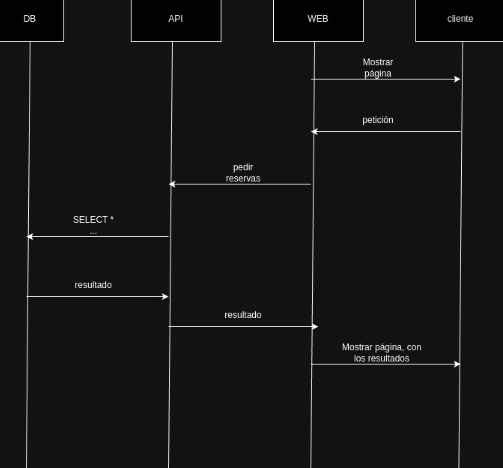
\includegraphics{estructura}

\subsection{Endpoints}

%cabanias

\textbf{Endponint}:/cabanias

metodo: GET

recibe: no se reciben parámetros


\textbf{Endpoint}: /cabanias/calendario/<string:cabania-id>

metodo: GET

recibe: no se reciben parámetros


\textbf{Endpoint}: /cabanias

metodo: POST 

recibe:
\{"secreto":...,"id":...,"nombre":..., \newline
"descripcion":...,"cap-max":...,"precio-noche":...\}


\textbf{Endpoint}: /cabanias/<string:id>

metodo: PATCH 

recibe: \{"secreto":...,
"nombre":...,"descripcion":...,
"cap-max":...,"precio-noche":...\}

metodo: DELETE

recibe: id (por URI)


%reservas


\textbf{Endpoint}: /reservas

metodo: GET

recibe:

\{"codigo-reserva": codigo-reserva,"nombre-cliente": nombre-cliente,

"cliente-id": cliente-id,"email": email,

"telefono": telefono, "fecha-ingreso": fecha-ingreso,

"fecha-egreso": fecha-egreso,"precio-total": precio-total\}


\textbf{Endpoint}: /reserva

metodo: GET

recibe: \{"cliente-id": cliente-id|pasaporte,"nombre-cliente" : nombre-cliente\}


\textbf{Endpoint}: /crear-reserva

metodo: POST

recibe: \{"cabania-id" : id,"fecha-ingreso" : "aaaa-mm-dd",

"fecha-egreso" : "aaaa-mm-dd","nombre-cliente" : "nombre-cliente",

"cliente-id": cliente-id,"telefono": telefono,

"email" : "example@example.com"\}


\textbf{Endpoint}: /reserva/<int:id>

metodo: DELETE

recibe:
\{"email" : example@mail.com\}

Si "email" es proporcionado, la reserva del cliente con el codigo de reserva 'id', sera eliminada.


\textbf{Endpoint}: /reserva/<int:id>

metodo: PATCH

recibe: \{"secreto" : passw\}

luego se puede modificar lo que se quiera de la reserva

%imagenes

\textbf{Endpoint}: /imagenes

metodo: GET

recibe:\{"secreto" : passw, "cabania-id" : id *opcional*\}

\textbf{Endpoint}: /crear-imagen

metodo: POST

recibe:

\{"secreto" : passw, "cabania-id" : id, *opcional*

"link" : url-img,"descripcion" : portada\}

\textbf{Endpoint}: /imagen

metodo: DELETE

recibe: \{"secreto" : passw, "link" : url\}

\href{https://github.com/MaxiFttInst/UBA_TP_IDS/blob/api/api/app.py}{API del proyecto}



























\section{Plan de actividades}

La creación de software se enfocó en la división de tareas desde el principio y la creación de una estructura que sustentaría todo el proyecto. Primero y principalmente creamos una ilustración que explicaba graficamente la forma en que sería el proyecto. Con el tiempo, esta ilustración se modificó en función de las tareas que surgían y las habilidades de cada miembro del equipo o su desempeño con respecto a las propuestas. 

La metodologia que se utilizo fue mediante una comunicacion activa para aclarar la planificacion de los objetivos y analizar en cada encuentro la realizacion de dichas actividades, donde se acordo que uno de los objetivos principales para llevar a cabo era el diseño que iba a presentar la pagina, para luego poder desarrollar la parte funcional y programar un entorno de desarrollo utilizando tecnologias para el backend. Después de haber cumplido con la importante tarea de haber trabajado en el Backend y en el Frontend quedaba poner a prueba y asegurar que tuviera un funcionamiento optimo para la experiencia del usuario, ya que la pagina debía cumplir con las funciones recientemente hechas y, por otro lado, la interfaz del usuario debía ser intuitiva y fácil de usar para así poder corregir y ajustar los errores que se presentaban.

Las herramientas que tuvimos a nuestro favor y para llevar a cabo el plan de actividades fue el gestor de proyectos \href{https://trello.com/b/gpuunRxX/tp-ids}{Trello}, donde pudimos listar las tareas entre los integrantes y asi tener un seguimiento de cada una. El desarrollo de la pagina lo logramos hacer gracias a la implementación de Git y \href{https://github.com/MaxiFttInst/UBA_TP_IDS}{GitHub}, y otros programas como Visual Studio Code, MySQLite, Docker, entre otros.

Los integrantes del proyecto contaron con una división de roles y responsabilidades que tuvieron que cumplir como Desarrolladores de Backend y Frontend, pero mas allá del rol principalmente impuesto se cada uno logró contribuir en cualquiera de las áreas, para ello realizábamos encuentros para charlar las cuestiones que se nos dificultaba, trabajar como equipo y documentar cualquier cambio que hiciéramos por medio de un grupo de Discord.

\subsection{Creación de frontend}

El desarrollo del Frontend fue una de las primeras tareas a realizar, ya que antes de comenzar la codificación se presentó un diseño y planificación de la estructura con la implementación de \textbf{HTML}, para la base de la pagina web, \textbf{CSS}, para definir el aspecto visual y aplicar estilos, y \textbf{JavaScript}, para agregar una interactividad y dinamismo.


\subsubsection{calendario}

La implementación de un calendario es importante a la hora de realizar las reservas, por que es la conexión entre el cliente y la funcionalidad, por lo que se tuvo que implementar desarrollo en el Front para la vista, como en el Back para la funcionalidad.


\subsection{Crear base de datos}


La base de datos es una parte crucial del trabajo ya que almacena toda la informacion de la pagina, ya sean las reservas, habitaciones e imagenes. Por lo que se implemento distintos diseños para realizar dicha base de datos como se pueden observar en las figuras \ref{fig:BD1} y \ref{fig:BD2}



\begin{figure}
    \centering
    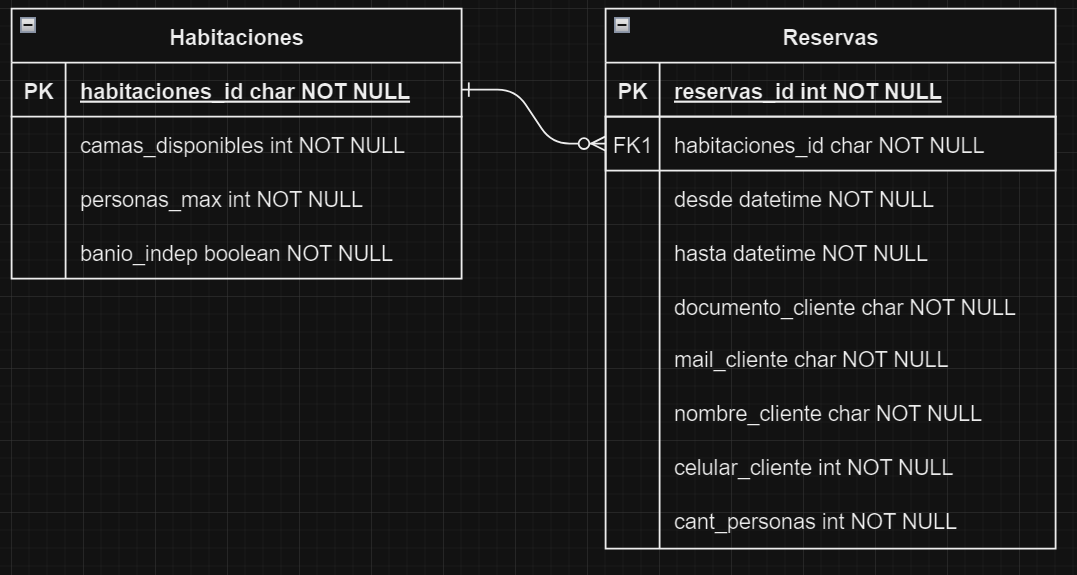
\includegraphics[width=0.75\linewidth]{images/base de datos 1.png}
    \caption{Idea principal de la Base de Datos}
    \label{fig:BD1}
\end{figure}


\begin{figure}
    \centering
    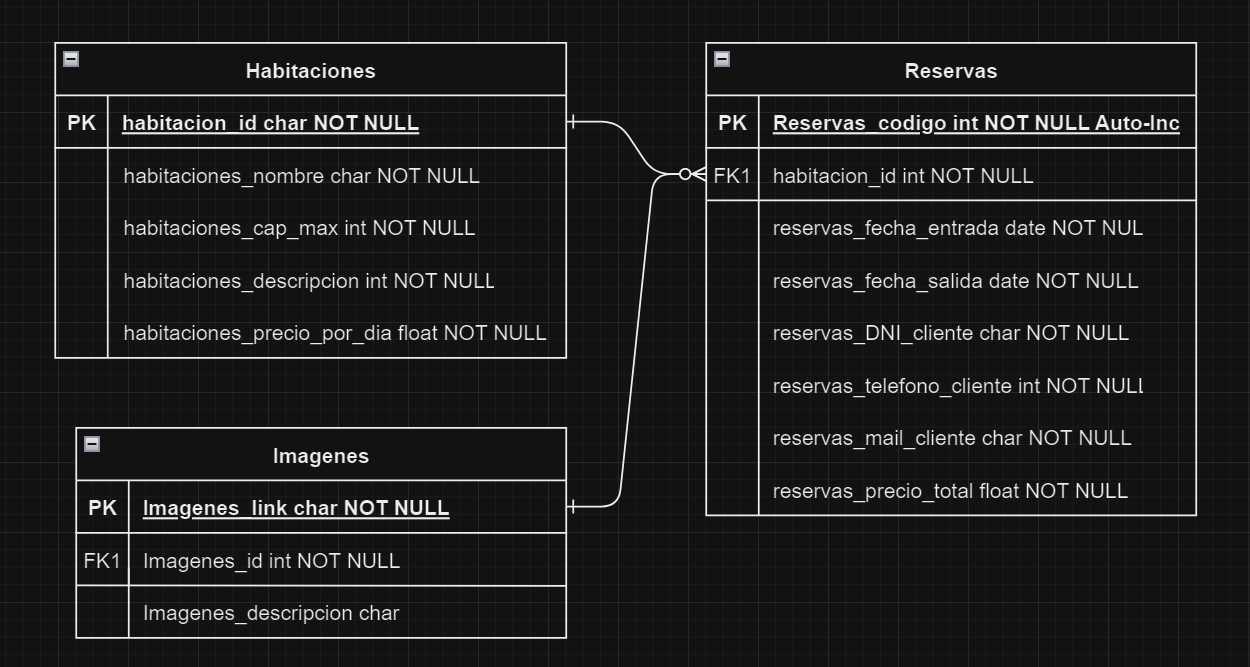
\includegraphics[width=0.75\linewidth]{images/base de datos final.png}
    \caption{Idea final de la Base de Datos}
    \label{fig:BD2}
\end{figure}


\subsection{Realizacion de requests}

El realizar los requests era necesario para todas las tablas de la base de datos de la pagina, ya sea para obtener los datos de las cabañas, como realizar la reserva o agregar alguna imagen de la cabaña, es por eso que se llevaron a cabo diferentes tareas donde se vieron implementadas cada una de estas funciones del CRUD (Create, Read, Update, Delete) para las diferentes tablas

\subsubsection{GET}

Los requests del tipo GET se utilizan para obtener datos del servidor, es por eso que se utilizo para saber que cabañas hay con disponibilidad, las reservas que hizo el mismo cliente o mismo para ver las imagenes implementadas.

\subsubsection{POST}

Los requests del tipo POST se utilizan para enviar datos al servidor, su implementación fue necesaria y esencial para realizar las mismas reservas y así poder guardarlas en la base de datos.

\subsubsection{PATCH}

El PATCH se utiliza para poder actualizar dichos datos del servidor, y fue necesario en el caso que se quiera modificar algún dato o el mismo día que se haya realizado la reserva.

\subsubsection{DELETE}

Los requests del tipo DELETE son utilizados para eliminar algún dato del servidor, para ello es de importancia su uso en el caso que se quiera cancelar una reserva a nombre de un cliente.

\subsection{Creación de backend (API)}

La Interfaz de Programacion de Aplicaciones es esencial para el Backend ya que es el gestor de lógica del servidor, sus operación junto a la base de datos y su comunicación con el Front. Su creación era necesaria para la conexión con la Base de Datos, las rutas, el propio servidor y los mismos Endpoints de la API en el cual estaban presentes todas las operaciones del CRUD.

\subsubsection{Deploy de la app y de la api}



\subsection{Cargado de imágenes en el drive}


Las imágenes son necesarias para poder generar una mejor experiencia con el usuario, ya que se muestran algunas de las cabañas en cuestión o mismo las instalaciones, actividades o servicio. Es por eso que se implemento el uso de \href{https://drive.google.com/drive/folders/1rzJS4rG295Mjmsm-0Xie7m3Bs8-YsvL0}{Google Drive} para cargar las imágenes, donde están todas subidas en una carpeta de llamada "Imágenes". Su implementación es necesaria por la buena gestión de archivos.


\subsection{Backoffice}

El Backoffice es una tarea que se precisaba para que el administrador sea capaz de modificar la pagina en el caso que sugiera algún cambio, ya sea en las imágenes, como en las reservas o las mismas cabañas. El administrador debe ser capaz de poder gestionar la información del mismo cliente en el caso que se precise para las reservas realizadas, o también debe tener la posibilidad de administrar la información de las mismas cabañas de la pagina, ya sea para implementar o quitar información. El administrador debe tener la posibilidad de modificar y gestionar la pagina de la posada con operaciones del CRUD de una forma sencilla.

\subsection{Conexion a la base de datos en pythonanywhere.}

Para exhibir la pagina de la posada se utilizó Pythonanywhere, el cual nos permite tener una conexion importante con los datos almacenados y la misma pagina.

\section{Hipotesis}

En esta sección se deberán volcar todas las hipótesis y supuestos que se hayan tomado en el alcance del trabajo. Recordar que las mismas no deben limitar o acotar el trabajo solicitado.
\section{Abstract}


Desde un principio decidimos elegir este desafío por que nos pareció adecuado para utilizar lo que aprendimos sobre el tema y pensamos que podía ser buena practica, ya que también para crear la página era necesario la investigación en profundidad de los temas enseñados.


El proyecto de la página web para "Posada Byteados" busca no solo establecer una presencia digital atractiva, sino también mejorar la experiencia del cliente mediante un sistema de reservas intuitivo y brindar toda la información necesaria. Se organizó con cuidado y atención a los detalles para garantizar todo el funcionamiento de la pagina sea estable.


Tanto en el Frontend como en el Backend se resolvieron y ajustaron numerosos problemas durante el trabajo, que incluyeron problemas visuales o problemas que el cliente no notaba, pero pudimos solucionarlos y estar satisfechos con lo que pudimos hacer.

\hspace{5cm}

English:


From the beginning we decided to choose this challenge because it seemed appropriate to use what we learned about the subject and we thought it could be good practice, since also to create the page it was necessary to research in depth the topics taught.

The website project for "Posada Byteados" seeks not only to establish an attractive digital presence, but also to improve the customer experience through an intuitive booking system and provide all the necessary information. It was organized with care and attention to detail to ensure the site's stable operation.

On both the frontend and backend numerous issues were resolved and adjusted during the work, which included visual issues or issues that the client didn't notice, but we were able to solve them and be satisfied with what we were able to do.









\end{document}
